\documentclass{article}
\usepackage[utf8]{inputenc}
\usepackage{graphicx}
\usepackage{amsfonts}
\usepackage{amsmath}

\author{Alessandro Messori, Daria Preda, Simone Tagliente}



\title{ \normalsize \textsc{PROJECT REPORT}
		\\ [2.0cm]
		\\
		\LARGE \textbf{\uppercase{MIDDLEWARE TECHNOLOGIES FOR DISTRIBUTED SYSTEMS}}
		\HRule \\ [0.5cm]
		\normalsize  \vspace*{5\baselineskip}}
\begin{figure}
	\centering
	
\includegraphics[width=0.5\linewidth]{resources/logo_polimi.png}
\end{figure}

\author{
        \textit{Authors:} \\
		Alessandro Messori \\
            Daria Preda \\  
            Simone Tagliente \\ 
            \\
            \\
            \textit{Professors:}\\
            Luca Mottola \\
            Alessandro Margara
            }

\begin{document}

\maketitle

\pagebreak

\tableofcontents

\pagebreak

\section{Project 1: Simulation and Analysis of Noise Level}
\subsection{Introduction}
The project is about designing and implementing a system that monitors the level of noise in a country that is divided into regions. Each region must provide data through sensors (either real or virtual) or a computer simulation (if the actual sensor data is not available). The data is collected into a proper back-end that performs data cleaning and enrichment on the sensor readings.
\subsection{Architecture}
\subsubsection{The Contiki Virtual Sensors}
The IoT system is developed and tested using COOJA simulator. In each region are deployed multiple border routers and sensors. 
\begin{figure}[htp]
	\centering
	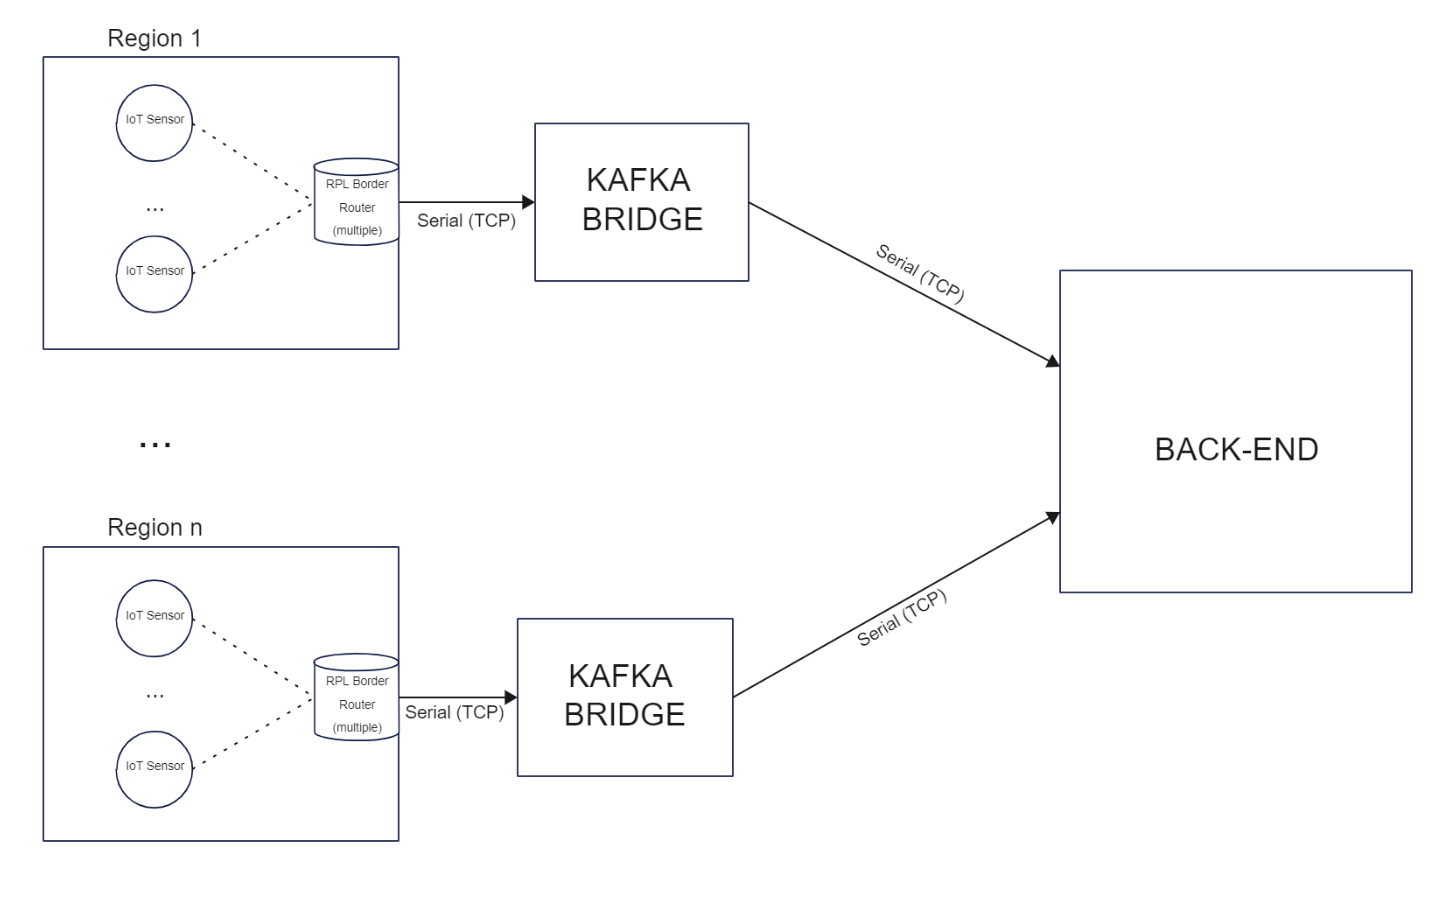
\includegraphics[width=0.9\linewidth]{resources/contiki_project_1.png}
	\caption{Example: 8 rooms, 2 sensors per room.}
	\label{fig:client_server_diag}
\end{figure}
\\
\\
Both the IoT devices run a single protothread. The sensor's protothread handles both the MQTT FSM (finite state machine) and the storing of the noise measurements. In the case of the border routers, the protothread handles a simple web server that allows the nodes to connect to the rest of the internet and publish on MQTT. The sensors publish one message every 10 seconds, as specified in the project description, in a single topic \texttt{"/iot/noise/json"}.
\\
\\
We used a script in javascript whose integration is natively provided by COOJA, to write to the serial interface of each sensor, which is in charge to read the value and store it in its memory. The data structure chosen is a simple queue of float which allows keeping a sliding window used to compute the average of the last six readings. Messages are published using the JSON format with this specific structure:
\begin{itemize}
    \item sensorID: int
    \item latitude: float
    \item longitude: float
    \item noise value: float
    \item timestamp: int
    \item threshold exceeded: int (0 or 1)
\end{itemize}
In the event that the threshold is exceeded by the computed average, the noise value field is substituted with a string which contains the representation of the queue
The latitude, the longitude and the noise level are sent through the serial interface to each sensor. The values are read through the javascript from a file containing a dataset of the Sensor Community website.
Each border router is associated with a producer running a bridge that subscribes to the MQTT topic and publishes messages into the Kafka topic \texttt{raw\_noise\_readings} .

\subsubsection{The Akka Simulation}

To simulate noise measurements we used the Akka model. We define three types of Actors: Noise Actors (Person or Vehicle) and Sensor, which are defined by their positions (latitude and longitude). The Person and Vehicle objects generate random noise data based on some certain thresholds. The Sensor objects act also as a Kafka Producer to send the readings received from the Noise Actors. 
\\
\\
Between the Actors, there are two types of messages used: RequestReadingMessage sent from Sensor to the Noise Actors, and NoiseReadingMessage sent from Noise Actors to the Sensor as a response. 
\\
\\
All the objects are initialized to a position close to each other at the beginning of the simulation. Noise Objects receive a request from a Sensor to generate data and send the reading only if the sensor it's in the area of action. The Actors also move at each iteration of the simulation at a fixed speed.
\\
\\
The Sensor keeps a list of readings and constructs the messages which are later sent to the Kafka Platform. The simulated noise reading messages respect the same format as the Contiki Virtual Sensors. 

\begin{figure}[htp]
	\centering
	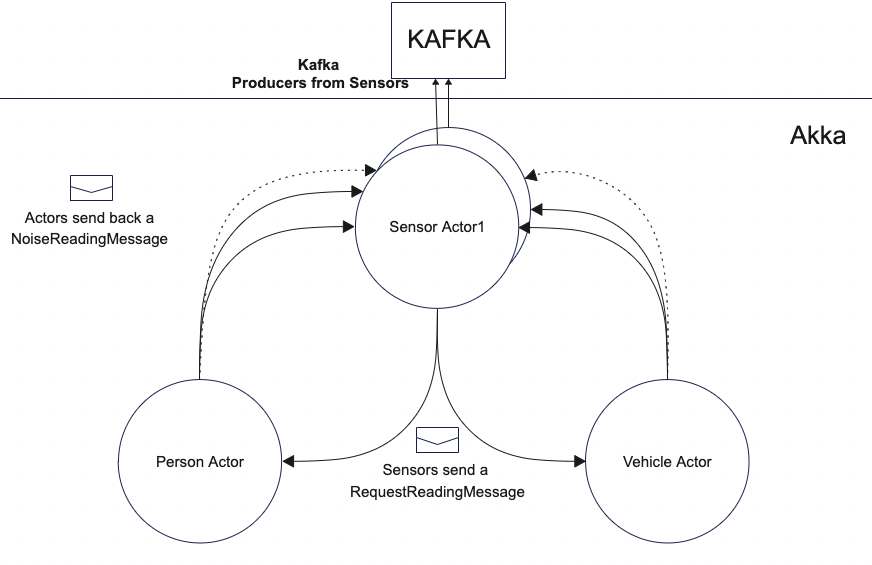
\includegraphics[width=0.9\linewidth]{resources/akka_archi.png}
	\caption{Example: 1 Person Actor and 1 Vehicle Actor communicating with a Sensor}
	\label{fig:akka_archi}
\end{figure}


\subsubsection{The Backend Platform}
The incoming data streams from the Contiki Virtual Sensors and the Akka Simulation are initially stored in their raw version inside a Kafka Topic called "raw\_noise\_readings", then a Spark Streaming Job performs a cleaning operation in order to delete corrupted or invalid data from the raw stream and saves the result in the "clean\_noise\_readings" topic. 
\\
Finally, a second Spark Streaming job reads the clean noise readings and enriches them by associating each one of them with the closest Point of Interest (this step is performed by joining the data stream with a static POI dataset read from a CSV file) and then storing the result of the computation in CSV files for permanent storage. 

\clearpage

\begin{figure}[htp]
    \centering
    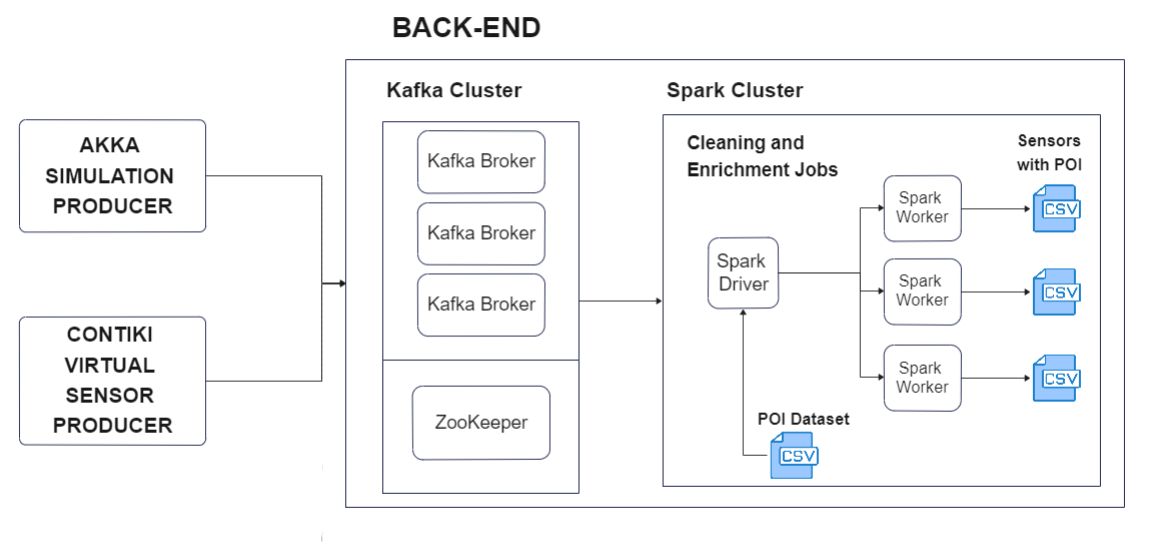
\includegraphics[width=0.9\linewidth]{resources/project1_backend_diagram.png}
    \caption{The Backend Architecture Diagram}
\end{figure}

\subsection{Design Choices}
\subsubsection{The IoT Virtual Sensors: Contiki-NG}
We have chosen Contiki-NG to implement our sensor due to the fact that it is designed for IoT devices. It allows us to deploy the sensor using energy-efficient platforms such as ARM Cortex-M3/M4 and the Texas Instruments MSP430 and provide IPv6 compatibility. 
\\
Since the only task of the sensor is to report the noise readings to the backend, we chose a publish/subscribe protocol as a communication paradigm. For the implementation we used MQTT. It provides a suitable lightweight protocol for small devices with low memory and low processing power and high scalability of the network.


\subsubsection{The Noise Simulation: Akka}
The reasoning behind choosing Akka for the simulation relies on the idea of actors and communication between these objects. The Actor Model of Akka allows us to create multiple objects that can interact by sending messages, which is exactly what happens in sensor-based communication. We can easily model different types of sensors as different Actors.
\\
\\
A noise sensor receives multiple messages from other objects (such as vehicles and persons) and should be able to work in a concurrent environment to process them. The scalability is also an important factor since the key of the simulation is to be dynamic: the sensor should be able to communicate with many objects which are moving around and can enter its action area.


\subsubsection{The Backend Platform: Kafka and Spark}
Our main objective when we were designing the backend platform was to build a scalable system capable of storing and processing large quantities of data coming in real-time from thousands of sources while at the same time being easily extended with analytical scripts.
\\
\\
For the processing engine, our choice was Kafka, we felt that the best way to model the sensor readings would be as a stream of values that can be processed in near real-time as they are generated and then stored for further processing, and Kafka allows us to implement these requirements easily.
\\
\\
The choice for the processing framework landed on Spark, it has great scalability and parallel processing capabilities, and it natively supports joining streams of real-time data with static datasets, which are key requirements for implementing the cleaning and enriching functionalities
\\
\\
The other alternatives we considered for processing the data were:
\begin{itemize}
    \item Akka, but its Actor based model didn't seem the best fit for our use case, and we felt it would be harder and less efficient to perform stream processing and dataset joining wrt Spark;
    \item MPI, but similarly to Akka we feared that we wouldn't have the same ease of use and access to high-level features that Spark can offer and that are incredibly useful for data cleaning and enrichment operations.
\end{itemize}

\pagebreak

\section{Project 2: Smart Buildings and Neighborhoods}
\subsection{Introduction}
The project is about designing and deploying a system able to manage IoT sensors and actuators in several buildings of possibly different neighbourhoods. Sensors deployed in a room periodically monitor environmental data, such as temperature and humidity. Such data is elaborated through the Edge-Computing paradigm by actuators whose task is to check whether the environmental data is below a specific threshold and activate an HVAC controller if the humidity or temperature falls outside of a certain range. 

%%Such data is sent and to the back-end which performs simple computations to check whether the temperature and the humidity are below a specific threshold and eventually activate the HVAC controller.

\subsection{Architecture}
\subsubsection{Implementation of Contiki-NG}
The IoT system is developed and tested using COOJA simulator. We design our network with a specific topology:
\begin{itemize}
    \item squared rooms of fixed dimension
    \item from 2 to 4 sensors positioned at the corners of a single room 
    \item one border router for every four rooms (two of them are shared with another border router)
\end{itemize}
As shown in Figure 1, each sensor is covered by at least 2 border routers to guarantee a higher level of fault tolerance of the system.

\begin{figure}[htp]
	\centering
	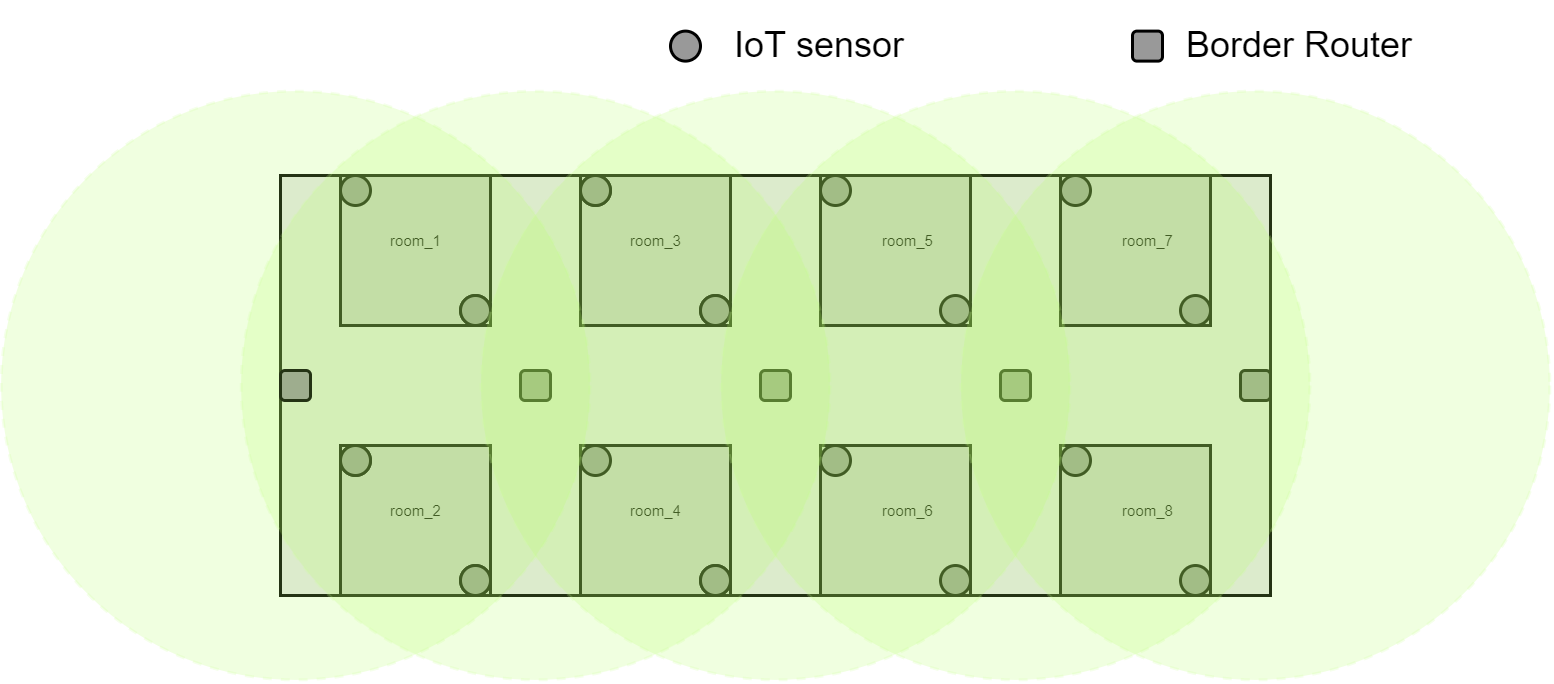
\includegraphics[width=\linewidth]{resources/building_example_1.drawio.png}
	\caption{Example: 8 rooms, 2 sensors per room.}
	\label{fig:client_server_diag}
\end{figure}
\clearpage
\\
Each IoT device runs a single protothread. In the case of the IoT sensors, the protothread handles both the MQTT FSM (finite state machine) and the storing of the temperature and humidity measurements. In the case of the border routers, the protothread handles a simple web server that allows the nodes to connect to the rest of the internet and publish on MQTT.
\\
The MQTT topics are differentiated by room and building, their general structure is \texttt{/iot/building\_(buildingID)/room\_(roomID)/json} where buildingID and roomID are incrementally generated and assigned to each sensor based on their position. The differentiation of the topics is useful to handle the environmental data of each room and building separately.
\\
\\
The messages produced by the IoT sensors have a JSON format that makes them easy to parse. Their structure is the following:

\begin{itemize}
    \item Uptime $(seconds)$
    \item Humidity value $(kg/m^3)$
    \item Temperature value $(C°)$
\end{itemize}
We used a script in javascript whose integration is natively provided by COOJA to set the building and the room associated with each mote and to send them periodically the measurements which are read from a file found in the datasets of the Sensor Community website.
\subsubsection{The Node-Red Actuators}
In order to increase the system's fault tolerance, we provided each of the rooms in the building with 2 actuators running a Node-Red flow. 
The first actuator is the main one and it's responsible for processing the MQTT readings coming from the Contiki sensors and turn on and off the heating/cooling system if needed. 
\\
The main actuator also periodically publishes a message to a heartbeat MQTT topic specific to its room. 
The backup actuator listens to both the MQTT heartbeat and readings topic associated with its room but stays idle until a certain amount of time passes (in our case 30 seconds) without receiving any heartbeat message from the main actuator. In that case, the backup actuator assumes the role of processing the sensor readings and consequently managing the AC system until the main one gets reactivated.  
\\
\begin{figure}[htp]
	\centering
	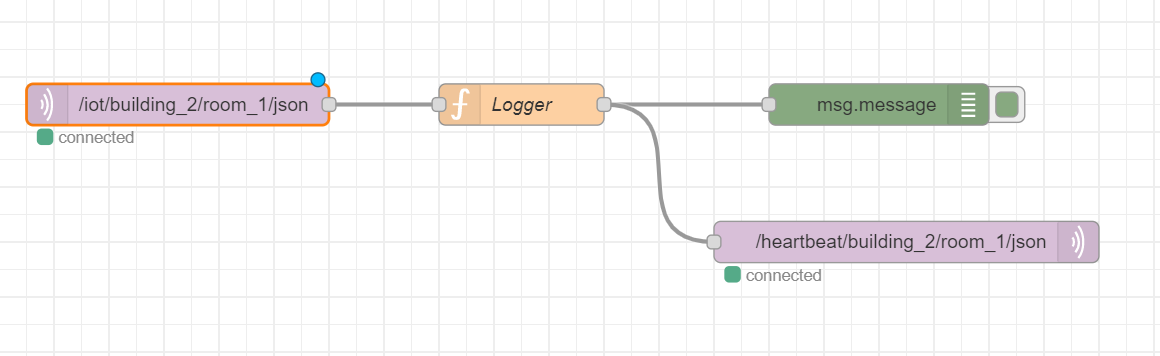
\includegraphics[width=\linewidth]{resources/mainActuator.png}
	\caption{Node Red Main Actuator}
	\label{fig:client_server_diag}
\end{figure}
\\
\begin{figure}[htp]
	\centering
	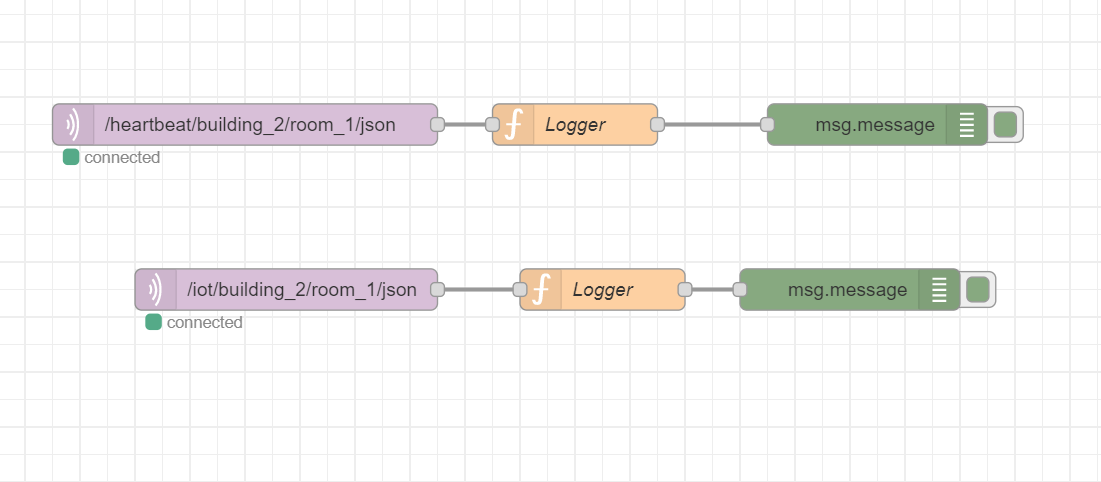
\includegraphics[width=\linewidth]{resources/backupActuator.png}
	\caption{Node Red Backup Actuator}
	\label{fig:client_server_diag}
\end{figure}
\pagebreak
\subsection{Design Choices}
\subsubsection{Why Contiki-NG}
We decide to use the Contiki-NG operating system to implement the IoT devices since it can be run on different platforms based on energy-efficient architectures (e.g. ARM Cortex-M3/M4 and the Texas Instruments MSP430) and it provides an RFC-compliant, low-power IPv6 communication stack, enabling Internet connectivity.
\linebreak
\linebreak
We chose MQTT as a communication paradigm since it is asynchronous and fits well for our needs: the IoT sensors periodically publish their measurements on a specific topic and there is no need for them to be coupled to subscribers. Thus, MQTT allows our system to be easily scalable and power-efficient and to have a dynamic topology of the network.

  
\subsubsection{Node Red over MPI for the actuators}
For the logic of the actuators, we chose Node Red since it improves latency and performance by moving the computation close to our interest. Another advantage is the ease of integration with MQTT which is harder to be acquired with MPI, a lower-level code model. Node-red is specially made for binding together hardware devices and online services, which is our case with actuators and MQTT. 
\\
\\
Even if MPI is suitable for obtaining high performance and the actuators can run a full-fledged OS, in our IoT environment we focus on the latency of communication and less on performing complex computations in parallel. 

\end{document}
